%% NYU PhD thesis format. Created by Jos� Koiller 2007--2008.

%% Use the first of the following lines during production to
%% easily spot "overfull boxes" in the output. Use the second
%% line for the final version.
%\documentclass[12pt,draft,letterpaper]{report}
\documentclass[12pt,letterpaper]{report}

%% Replace the title, name, advisor name, graduation date and dedication below with
%% your own. Graduation months must be January, May or September.
\newcommand{\thesistitle}{A comparison of schemes for the numerical approximation of the gyroaveraging operator}
\newcommand{\thesisauthor}{Oren Bassik}
\newcommand{\thesisadvisor}{Professor Antoine Cerfon}
\newcommand{\graddate}{May 2021}
%% If you do not want a dedication, scroll down and comment out
%% the appropriate lines in this file.
\newcommand{\thesisdedication}{To my dog Weierstra\ss, with affection.}

%% The following makes chapters and sections, but not subsections,
%% appear in the TOC (table of contents). Increase to 2 or 3 to
%% make subsections or subsubsections appear, respectively. It seems
%% to be usual to use the "1" setting, however.
\setcounter{tocdepth}{1}

%% Sectional units up to subsubsections are numbered. To number
%% subsections, but not subsubsections, decrease this counter to 2.
\setcounter{secnumdepth}{3}

%% Page layout (customized to letter paper and NYU requirements):
\setlength{\oddsidemargin}{.6in}
\setlength{\textwidth}{5.8in}
\setlength{\topmargin}{.1in}
\setlength{\headheight}{0in}
\setlength{\headsep}{0in}
\setlength{\textheight}{8.3in}
\setlength{\footskip}{.5in}

%% Use the following commands, if desired, during production.
%% Comment them out for final version.
%\usepackage{layout} % defines the \layout command, see below
%\setlength{\hoffset}{-.75in} % creates a large right margin for notes and \showlabels

%% Controls spacing between lines (\doublespacing, \onehalfspacing, etc.):
\usepackage{setspace}

%% Use the line below for official NYU version, which requires
%% double line spacing. For all other uses, this is unnecessary,
%% so the line can be commented out.
%\doublespacing % requires package setspace, invoked above

%% Each of the following lines defines the \com command, which produces
%% a comment (notes for yourself, for instance) in the output file.
%% Example:    \com{this will appear as a comment in the output}
%% Choose (uncomment) only one of the three forms:
%\newcommand{\com}[1]{[/// {#1} ///]}       % between [/// and ///].
\newcommand{\com}[1]{\marginpar{\tiny #1}} % as (tiny) margin notes
%\newcommand{\com}[1]{}                     % suppress all comments.

%% This inputs your auxiliary file with \usepackage's and \newcommand's:
%% It is assumed that that file is called "definitions.tex".
%%
%% Place here your \usepackage's. Some recommended packages are already included.
%%

% Graphics:
\usepackage[final]{graphicx}
%\usepackage{graphicx} % use this line instead of the above to suppress graphics in draft copies
%\usepackage{graphpap} % \defines the \graphpaper command

% Indent first line of each section:
\usepackage{indentfirst}

% Good AMS stuff:
\usepackage{amsthm} % facilities for theorem-like environments
\usepackage[tbtags]{amsmath} % a lot of good stuff!

% Fonts and symbols:
\usepackage{amsfonts}
\usepackage{amssymb}
\usepackage{physics}

\usepackage{tikz}
\usetikzlibrary{patterns,shapes.arrows}
\usepackage{pgfplots}
\pgfplotsset{compat=newest}
\usepgfplotslibrary{external}
\usepgfplotslibrary{groupplots,dateplot}
\tikzexternalize


\usepackage[utf8]{inputenc}
\usepackage{pgfplots}
%\DeclareUnicodeCharacter{2212}{−}  %this breaks



% Formatting tools:
%\usepackage{relsize} % relative font size selection, provides commands \textsmalle, \textlarger
%\usepackage{xspace} % gentle spacing in macros, such as \newcommand{\acims}{\textsc{acim}s\xspace}

% Page formatting utility:
%\usepackage{geometry}

%%
%% Place here your \newcommand's and \renewcommand's. Some examples already included.
%%
\renewcommand{\le}{\leqslant}
\renewcommand{\ge}{\geqslant}
\renewcommand{\emptyset}{\ensuremath{\varnothing}}
\newcommand{\ds}{\displaystyle}
\newcommand{\R}{\ensuremath{\mathbb{R}}}
\newcommand{\Q}{\ensuremath{\mathbb{Q}}}
\newcommand{\Z}{\ensuremath{\mathbb{Z}}}
\newcommand{\N}{\ensuremath{\mathbb{N}}}
\newcommand{\T}{\ensuremath{\mathbb{T}}}
\newcommand{\eps}{\varepsilon}
\newcommand{\closure}[1]{\ensuremath{\overline{#1}}}
%\newcommand{\acim}{\textsc{acim}\xspace}
%\newcommand{\acims}{\textsc{acim}s\xspace}

%%
%% Place here your \newtheorem's:
%%

%% Some examples commented out below. Create your own or use these...
%%%%%%%%%\swapnumbers % this makes the numbers appear before the statement name.
%\theoremstyle{plain}
%\newtheorem{thm}{Theorem}[chapter]
%\newtheorem{prop}[thm]{Proposition}
%\newtheorem{lemma}[thm]{Lemma}
%\newtheorem{cor}[thm]{Corollary}

%\theoremstyle{definition}
%\newtheorem{define}{Definition}[chapter]

%\theoremstyle{remark}
%\newtheorem*{rmk*}{Remark}
%\newtheorem*{rmks*}{Remarks}

%% This defines the "proo" environment, which is the same as proof, but
%% with "Proof:" instead of "Proof.". I prefer the former.
%\newenvironment{proo}{\begin{proof}[Proof:]}{\end{proof}}



\makeatletter
\newcommand*{\mint}[1]{%
	% #1: overlay symbol
	\mint@l{#1}{}%
}
\newcommand*{\mint@l}[2]{%
	% #1: overlay symbol
	% #2: limits
	\@ifnextchar\limits{%
		\mint@l{#1}%
	}{%
		\@ifnextchar\nolimits{%
			\mint@l{#1}%
		}{%
			\@ifnextchar\displaylimits{%
				\mint@l{#1}%
			}{%
				\mint@s{#2}{#1}%
			}%
		}%
	}%
}
\newcommand*{\mint@s}[2]{%
	% #1: limits
	% #2: overlay symbol
	\@ifnextchar_{%
		\mint@sub{#1}{#2}%
	}{%
		\@ifnextchar^{%
			\mint@sup{#1}{#2}%
		}{%
			\mint@{#1}{#2}{}{}%
		}%
	}%
}
\def\mint@sub#1#2_#3{%
	\@ifnextchar^{%
		\mint@sub@sup{#1}{#2}{#3}%
	}{%
		\mint@{#1}{#2}{#3}{}%
	}%
}
\def\mint@sup#1#2^#3{%
	\@ifnextchar_{%
		\mint@sup@sub{#1}{#2}{#3}%
	}{%
		\mint@{#1}{#2}{}{#3}%
	}%
}
\def\mint@sub@sup#1#2#3^#4{%
	\mint@{#1}{#2}{#3}{#4}%
}
\def\mint@sup@sub#1#2#3_#4{%
	\mint@{#1}{#2}{#4}{#3}%
}
\newcommand*{\mint@}[4]{%
	% #1: \limits, \nolimits, \displaylimits
	% #2: overlay symbol: -, =, ...
	% #3: subscript
	% #4: superscript
	\mathop{}%
	\mkern-\thinmuskip
	\mathchoice{%
		\mint@@{#1}{#2}{#3}{#4}%
		\displaystyle\textstyle\scriptstyle
	}{%
		\mint@@{#1}{#2}{#3}{#4}%
		\textstyle\scriptstyle\scriptstyle
	}{%
		\mint@@{#1}{#2}{#3}{#4}%
		\scriptstyle\scriptscriptstyle\scriptscriptstyle
	}{%
		\mint@@{#1}{#2}{#3}{#4}%
		\scriptscriptstyle\scriptscriptstyle\scriptscriptstyle
	}%
	\mkern-\thinmuskip
	\int#1%
	\ifx\\#3\\\else_{#3}\fi
	\ifx\\#4\\\else^{#4}\fi  
}
\newcommand*{\mint@@}[7]{%
	% #1: limits
	% #2: overlay symbol
	% #3: subscript
	% #4: superscript
	% #5: math style
	% #6: math style for overlay symbol
	% #7: math style for subscript/superscript
	\begingroup
	\sbox0{$#5\int\m@th$}%
	\sbox2{$#5\int_{}\m@th$}%
	\dimen2=\wd0 %
	% => \dimen2 = width of \int
	\let\mint@limits=#1\relax
	\ifx\mint@limits\relax
	\sbox4{$#5\int_{\kern1sp}^{\kern1sp}\m@th$}%
	\ifdim\wd4>\wd2 %
	\let\mint@limits=\nolimits
	\else
	\let\mint@limits=\limits
	\fi
	\fi
	\ifx\mint@limits\displaylimits
	\ifx#5\displaystyle
	\let\mint@limits=\limits
	\fi
	\fi
	\ifx\mint@limits\limits
	\sbox0{$#7#3\m@th$}%
	\sbox2{$#7#4\m@th$}%
	\ifdim\wd0>\dimen2 %
	\dimen2=\wd0 %
	\fi
	\ifdim\wd2>\dimen2 %
	\dimen2=\wd2 %
	\fi
	\fi
	\rlap{%
		$#5%
		\vcenter{%
			\hbox to\dimen2{%
				\hss
				$#6{#2}\m@th$%
				\hss
			}%
		}%
		$%
	}%
	\endgroup
}


%% Cross-referencing utilities. Use one or the other--whichever you prefer--
%% but comment out both lines for final version.
%\usepackage{showlabels}
%\usepackage{showkeys}


\begin{document}
%% Produces a test "layout" page, for "debugging" purposes only.
%% Comment out for final version.
%\layout % requires package layout (see above, on this same file)

%%%%%% Title page %%%%%%%%%%%
%% Sets page numbering to "roman style" i, ii, iii, iv, etc:
\pagenumbering{roman}
%
%% No numbering in the title page:
\thispagestyle{empty}
%
\begin{center}
  {\large\textbf{\thesistitle}}
  \vspace{.7in}

  by
  \vspace{.7in}

  \thesisauthor
  \vfill

\begin{doublespace}
  A dissertation submitted in partial fulfillment\\
  of the requirements for the degree of\\
  Master of Science\\
  Department of Mathematics\\
  New York University\\
  \graddate
\end{doublespace}
\end{center}
\vfill

\noindent\makebox[\textwidth]{\hfill\makebox[2.5in]{\hrulefill}}\\
\makebox[\textwidth]{\hfill\makebox[2.5in]{\hfill\thesisadvisor\hfill}}
\newpage
%%%%%%%%%%%%% Blank page %%%%%%%%%%%%%%%%%%
\thispagestyle{empty}
\vspace*{0in}
\newpage

%%%%%%%%%%%%%% Dedication %%%%%%%%%%%%%%%%%
%% Comment out the following lines if you do not want to dedicate
%% this to anyone...
%\vspace*{\fill}
%\begin{center}
 % \thesisdedication\addcontentsline{toc}{section}{Dedication}
%\end{center}
%\vfill
%\newpage
%%%%%%%%%%%%%% Acknowledgements %%%%%%%%%%%%
%% Comment out the following lines if you do not want to acknowledge
%% anyone's help...
%\section*{Acknowledgements}\addcontentsline{toc}{section}{Acknowledgements}
%%% Write your acknowledgements in this file. If you do not want to acknowledge anyone,
%% you can delete this file and comment out the corresponding part in the "thesis.tex"
%% file.
%
I am indebted to Prof. Antoine Cerfon, for his constant support and inspiration.     

%\newpage
%%%% Abstract %%%%%%%%%%%%%%%%%%
\section*{Abstract}\addcontentsline{toc}{section}{Abstract}
%% Write your abstract here.
%

The gyroaverage operator, or 2d spherical mean transform, transforms a bivariate function by averaging values over circles of (potentially large) radius.  This operator has applications in plasma simulation as well as medical imaging, and its naive calculation for large radii is not well-tuned for modern, cache-sensitive processors.  We implement and benchmark a variety of schemes for calculating gyroaverages in the 2D, compactly supported non-periodic setting. Schemes implemented include bilinear spline collocation, bicubic spline collocation, padded (bivariate) FFT interpolation, and bivariate tensor Chebyshev interpolation. In particular we quantify the impact of shared-memory parallelism and the use of GPU accelerators to speed up calculations, as well as the trade-off of accuracy vs computational cost, for both smooth functions and those with singularities.
\newpage
%%%% Table of Contents %%%%%%%%%%%%
\tableofcontents

%%%%% List of Figures %%%%%%%%%%%%%
%% Comment out the following two lines if your thesis does not
%% contain any figures. The list of figures contains only
%% those figures included withing the "figure" environment.
\listoffigures\addcontentsline{toc}{section}{List of Figures}
\newpage

%%%%% List of Tables %%%%%%%%%%%%%
%% Comment out the following two lines if your thesis does not
%% contain any tables. The list of tables contains only
%% those tables included withing the "table" environment.
\listoftables\addcontentsline{toc}{section}{List of Tables}
\newpage

%%%%% Body of thesis starts %%%%%%%%%%%%
\pagenumbering{arabic} % switches page numbering to arabic: 1, 2, 3, etc.
%% Introduction. If your thesis has no introduction, or chapter 1 is
%% meant to be the introduction, then comment out the lines below.
%\section*{Introduction}\addcontentsline{toc}{section}{Introduction}
%%% Write your introduction here.
%
%\part{First Part\label{part:one}}%
\section{Background\label{sec:Background}}



%In chapter~\ref{chap:one} we do this and that.



%In the latter chapters we\ldots

%% If your thesis has different "Parts", use commands such as the following:
%\part{First Part\label{part:one}}%
\chapter{Introduction\label{chap:one}}

\section{Background\label{sec:Background}}
Given a function $f$ taking real or complex values on some domain in $\mathbb{R}^2$, and an additional parameter specifying a radius $\rho$, define the gyroaveraging operator as
\[ \mathcal{G}(f)(x,y;\rho) = \frac{1}{2 \pi}\int_{0}^{2\pi} f(x+\rho \sin(\gamma), y + \rho \cos(\gamma)) \dd{\gamma}\]
%REFERENCES: Evans, Guadagni Thesis, wikipedia, other standard PDE books
This operator is a special case of what is called in various texts a spherical mean operator, peripheral mean operator,  or spherical Radon transform.  The spherical mean transform is defined for any dimension $n \geq 1$ as  
\[ \mathcal{J}(f)(\mathbf{x};\rho) = \frac{1}{\omega_n}\int_{\abs{\mathbf{y}}=1} f(x+\rho \mathbf{y}) \dd{S(\mathbf{y})} = \mintlocal{-}_{\partial B(\mathbf{x}, \rho)} f(\mathbf{y})\dd{S(\mathbf{y})}\]
%TODO expand on terms above
This operator is introduced in many PDE textbooks (see, for instance, \cite[p. 67]{evansPDE}), among other applications, to solve the wave equation in $n$ dimensions.  Our interest in the numerical calculation of the 2D case, as well as the name ``gyroaverage", comes from an application in plasma physics: solving the ``Vlasov-Poisson" equations to simulate a beam of charged particles in a cyclotron. While a detailed derivation is out of the scope of this thesis, and is described in detail in \cite{guadagniThesis}, a very brief description of the scheme is given (in \cite{guadagniThesis}) as:
%REFERENCE: guadagni & cerfon, and [4] in guadagni thesis (Earlier cerfon paper)

\begin{quote} Briefly, our method of solution of the VPE consists of the following steps: (1) calculate $\mathcal{G}$f via various numerical
	algorithms, (2) compute $\chi$ with a free-boundary Poisson solver, and (3) time-advance $f$ in the
	Vlasov equation.
\end{quote}
The Poisson solver and time-stepping parts of the solver are well-studied and have many well-known schemes (as well as many freely available implementations); meanwhile the gyroaveraging operator is being applied inside the time-stepping loop and suffers from (as is apparent from the definition) ``everywhere-to-everywhere" dependence.  Thus it is reasonable to expect gains from speeding up the gyroaveraging as the lowest hanging fruit in improving this particular solver. 

Another application  (described in \cite{gorner2012} and \cite{gorner2015}) is in the field of thermoacoustic tomography.  Very briefly, an electromagnetic radiation source is applied to a body of biologic tissue, which generates heat pulses in the tissue; this in turn causes small, temporary expansions.  These expansions radiate outwards as sound waves, and are detected at the boundary of the tissue by an array of transducers.  The reconstruction of an image from the transducer signals is, mathematically, a problem of inverting the spherical mean transform.  One angle of attack for the inverse problem is via iterative methods, which rely on applying the forward transform to repeatedly refine potential inverses; for these methods efficient and scalable algorithms for the forward transform translate into gains for the inverse.  
%Torsten Gorner thesis
%wikipedia on thermoacoustic imaging


%figure~\ref{fig:afigure}.
%\begin{figure}[htb]
%  \begin{center}
%    \emph{This statement is false.}
%  \end{center}%
%\caption[This alternate caption appears in the list of figures.]{This is the
%caption that appears under the figure. It may be quite long---you wouldn't want
%such a long caption to appear in the ``list of figures''.}
%\label{fig:afigure}
%\end{figure}

%More blah, blah. There is nothing interesting about
%table~\ref{tab:atable} either.
%\begin{table}[htb]
%\caption[Strange rules.]{For some reason unfamiliar to me,
%typesetting rules require one to place captions above tables,
%but below figures. Go figure.}\label{tab:atable}
%  \begin{center}
%    \framebox{You could put a table here. I won't.}
%  \end{center}
%\end{table}

%TODO REPLACE WITH CHAPTER REFERENCES below
\section{Outline\label{Outline}}
In the remainder of this paper, we will focus on the forward gyroaveraging operator alone, in a 2D setting.  We assume that we are in the context of a numerical solver, and that we have access to function values alone (and not an analytic representation), and that our domain of interest is bounded (i.e. we are gyroaveraging functions of compact support.)  

Chapter \ref{chap:background} will recall some basic facts needed for the rest of the paper, including: Fourier analysis, Chebyshev approximation theory and spline approximation, as well as basic properties of the spherical mean transform.

Chapter \ref{chap:discretizations} will describe the four different discretizations which we implemented, and the mathematical operation of applying the gyroaverage operator onto each.  In the case of smooth functions, we present some error estimates.

Chapter \ref{chap:DesignConsiderations} adds implementation details, and addresses design considerations from the computer science perspective.  Included is a very brief overview of the API implemented.  
%including details on memory usage, asymptotic runtime complexity, CPU multicore parallelism, GPU parallelism, and the extent and nature of precomputation necessary.

Chapter \ref{chap:NumericalResults} presents numerical results; we start by defining four functions with different salient features and in each case analyze converge and calculation speed, for each implemented algorithm.

%Chapter 6 is a brief summary of the API implemented; we have tried to make a user-friendly self-contained C++ header-only library with dependencies on publicly available free software.  In addition via RAII and templates we allow the user fine control over memory usage with no overhead in interface complexity, and the ability to pass any sort of callable object.

Chapter \ref{chap:Conclusion} summarizes the numerical results and outlines areas for further improvement and investigation.


\chapter{Background\label{chap:two}}

We use this chapter to record some basic facts we will use later.  Mainly we will be quoting from references.

\section{Harmonic Analysis\label{sec:Harmonic}}
%reference Zygmund, Boyd Spectral methods, Trefethen spectral methods
The below follows the notation and presentation from (REFERENCE: ATAP for periodic functions).  Let $f$ be a Lipschitz continuous periodic function defined on $[0,2 \pi]$.  Then $f$ is associated to a Fourier series
\[  f(t) = \sum_{k=-\infty}^{k=\infty} c_k e^{ikt}\]
where the coefficients are given by the formula
\[c_k = \frac{1}{2\pi}  \int_{0}^{2\pi} f(t) e^{-ikt} \dd{t}. \]
We can truncate this expansion:
\[f_n(t) = \sum_{k=-n}^{n} c_k e^{ikt}\]
which is an approximation to $f$, the ``degree $n$ trigonometric projection" of $n$.\\
In practice, we may not have access to the exact coefficients $c_k$, but must rely only on values of $f$ sampled at $N$ points, generally equispaced in $[0,2\pi]$. Let $f_j = f \left( \frac{2 \pi j  }{N} \right) $  Then we can use the formula
\[  \tilde{c}_k = \frac{1}{N} \sum_{j=0}^{N-1} f_k e^{-ikt}\] 
 which gives, via the same truncated expansion as above, the ``trigonometric interpolant" $p_n$ to $f$.   \\
 
 Now, if $f$ satisfies some smoothness condition, a standard argument involving repeated integration by parts yields the below error bounds.  This is Theorem B.2 in (REFERENCE: ATAP for periodic functions)
 
 \newtheorem*{ATAPB-2}{Theorem B.2} 
 \begin{ATAPB-2}If $f$ is $\nu \geq 1$ times differentiable and $f^{(\nu)}$ is of bounded 
 variation $V$ on $[0,2\pi]$, then its degree $n$ trigonometric projection and interpolant satisfy
 \[ \norm{f - f_n}_\infty \leq \frac{V}{\pi \nu n^\nu}, \quad \norm{f - p_n}_\infty \leq \frac{2V}{\pi \nu n^\nu} \]
 If $f$ is analytic with $\abs{f(t) \leq M}$ in the open strip of half-width $\alpha$ around the real axis in the complex $t$-place, they satisfy
 \[ \norm{f - f_n}_\infty \leq \frac{2Me^{-\alpha n}}{e^\alpha-1}, \quad \norm{f - p_n}_\infty \leq \frac{4M e^{-\alpha n}}{e^\alpha -1} \]
 \end{ATAPB-2}

\section{Harmonic Analysis of the Spherical Mean \label{sec:Harmonic2}}
Our interest in Fourier analysis is justified by the following calculation, which shows how the gyroaverage is greatly simplified in frequency space.  We focus on the bivariate case.  Suppose we have a Lipschitz continuous function $f$ on $\Omega = [0,2\pi]^2$, which is continuous and doubly periodic.  We have the Fourier series
\[ f(x,y) = \sum_{k=\infty}^{\infty} \sum_{\ell = \infty}^{\infty} c_{k,\ell} e^{2 \pi i (kx+\ell y)}  \]
where
\[ c_{k,\ell} = \int_{0}^{2 \pi} \int_{0}^{2 \pi} f(t_1,t_2) e^{-2 \pi i (kt_1 + \ell t_2)} \dd{t_1} \dd{t_2}\]

If we recall the definition of the gyroaverage
\[ \mathcal{G}(f)(x,y;\rho) = \frac{1}{2 \pi}\int_{0}^{2\pi} f(x+\rho \sin(\gamma), y + \rho \cos(\gamma)) \dd{\gamma}\]
We can ask what happens to a Fourier basis function under this operator.  Let
\[ f_{k, \ell} (x,y) = e^{2 \pi i (kx+\ell y)}   \]
Then
\[ \mathcal{G}(f_{k,\ell}) = \frac{1}{2 \pi}  \int_{0}^{2\pi} f(x+\rho \sin(\gamma), y + \rho \cos(\gamma)) \dd{\gamma} =  \]
\[  \frac{1}{2 \pi}  \int_{0}^{2\pi} e^{2 \pi i (k(x + \rho \sin \gamma) + \ell(y + \rho \cos \gamma))} \dd{\gamma} =   \frac{e^{2 \pi i (kx + \ell y)}}{2 \pi}\int_{0}^{2\pi} e^{2 \pi i \rho (k \sin \gamma + \ell \cos \gamma)} \dd{\gamma} =   \]
\[ f_{k,\ell} \frac{1}{2 \pi}\int_{0}^{2\pi} e^{2 \pi i \rho (k \sin \gamma + \ell \cos \gamma)} \dd{\gamma} \]
Next we use the identity $k \sin \gamma + \ell \cos \gamma = C \cos (\gamma + \phi)$, where $C = \sqrt{k^2 + \ell^2}$ and $\phi = \tan[-1](-\frac{k}{l})$.  The above is then 
\[ \mathcal{G}(f_{k,\ell}) = f_{k,\ell} \frac{1}{2 \pi} \int_{0}^{2 \pi} e^{2 \pi i \rho C \cos(\gamma + \phi)} = f_{k,l}  \cdot J_0(2 \pi \rho \sqrt{k^2 + \ell^2}) \]
Where $J_0(\cdot)$ is a Bessel function of the first kind, and the above is one form of the integral representation" found, e.g. in (REFERENCE: wikipedia). 
%or abramowitz/stegun).  
Applied to the Fourier series expansion of an arbitrary function $f$, we see that
\[\mathcal{G}(f)(x,y;\rho) = \sum_{k=\infty}^{\infty} \sum_{\ell = \infty}^{\infty}  J_0(2 \pi \rho \sqrt{k^2 + \ell^2}) c_{k,\ell} e^{2 \pi i (kx+\ell y)}   \] 
This is expected, as the gyroaverage is a form of convolution; in Fourier space the operator is computed simply by a multiplier that depends only on $(\rho$, $k$, $l)$.  This fact is true, with similar derivation and slightly different Bessel functions, for all dimensions and for continuous Fourier transforms as well.

%\[ \frac{e^{2 \pi i (kx + \ell y)}}{2 \pi}
%\int_{0}^{2\pi} \cos(2 \pi \rho k \sin \gamma + 2 \pi \rho \ell \cos \gamma) + i \sin(2 \pi %\rho k \sin \gamma + 2 \pi \rho \ell \cos \gamma) \dd{\gamma}
% \]





\section{Chebyshev Approximation\label{Chebyshev}}
A full review of Chebyshev polynomials and their use in approximation theory is beyond the scope of this paper.  For one who is comfortable with Fourier analysis, the easiest point of view is that to approximate a function $f$ on $[-1,1]$, wrap it around the unit circle by the transform
\[ \theta = \cos^{-1} x \]
Then $f(\cos(\theta))$ is a periodic, even function which is then subject to decomposition and approximation by (cosine) Fourier methods.  We quote 3 theorems from (REFERENCE : ATAP) which are analogous to the results for Fourier series above.

Define the Chebyshev polynomials as 
\[  T_k(x) = \cos(k \cos^{-1}(x))\]
Then any Lipschitz continuous function on $[-1,1]$ has a representation 
\[ f(x) = \sum_{k=0}^{\infty} a_k T_k(x) \]
with
\[ a_k = \frac{2}{\pi} \int_{-1}^{1} \frac{f(x) T_k(x)}{\sqrt{1-x^2}} \dd{x} \]
except that $\frac{2}{\pi}$ becomes $\frac{1}{\pi}$ for $k=0$.  
We can truncate this series and obtain 
\[ f_n(x) = \sum_{k=0}^{n} a_k T_k(x) \]
or, in analogy to the Fourier case, we can admit that in practice we may not have access to the integrals defining $a_k$.  Then we sample at Chebyshev nodes, $x_j = \cos \left(  \frac{j \pi}{n} \right)$ and interpolate to find coefficients $c_k$, such that\[p_n(x) =   \sum_{k=0}^{n} c_k T_k(x) \]
satisfies $p_n(x_j) = f(x_j)$.  (This interpolation is a discrete cosine transform, and is handled efficiently by FFT-based algorithms.)  Then we have the following theorems bounding the error of the above, quoted from ATAP.  We will not pause to define every term, and indeed Bernstein ellipses are somewhat technical.  The moral is that smoother functions will have faster convergence from interpolants than less smooth functions.
\newtheorem*{ATAP7-2}{Theorem 7.2 Convergence for differentiable functions}
\begin{ATAP7-2}
	For any integer $\nu \ge 0$, let $f$ and its derivatives through $f^{\nu -1}$ be absolutely continuous on $[-1,1]$ and suppose the $\nu$th derivative is of bounded variation $V$, then for any $n > \nu$, the Chebyshev projections satisfy 
	\[  \norm{f - f_n} \leq \frac{2V}{\pi \nu (n - \nu)\nu} \]
	and its Chebyshev interpolants satisfy
	\[ \norm {f- p_n} \leq \frac{4V}{\pi \nu (n-\nu)^{\nu}}\]
\end{ATAP7-2}
\newtheorem*{ATAP8-2}{Theorem 8.2 Convergence for analytic functions}
\begin{ATAP8-2}
	Let a function $f$ analytic in $[-1,1]$ be analytically continuable to the open Bernstein ellipse $E_\rho$, where it satisfies $\abs{f(x)}\leq M$ for some $M$.  Then for each $n \geq 0$ its Chebyshev projections satisfy 
	\[  \norm{f - f_n} \leq \frac{2 M \rho^{-n} }{\rho - 1} \]
	and its Chebyshev interpolants satisfy
	\[ \norm {f- p_n} \leq \frac{4 M \rho^{-n} }{\rho - 1}\]
\end{ATAP8-2}



%figure~\ref{fig:afigure}.
%\begin{figure}[htb]
%  \begin{center}
%    \emph{This statement is false.}
%  \end{center}%
%\caption[This alternate caption appears in the list of figures.]{This is the
%caption that appears under the figure. It may be quite long---you wouldn't want
%such a long caption to appear in the ``list of figures''.}
%\label{fig:afigure}
%\end{figure}

%More blah, blah. There is nothing interesting about
%table~\ref{tab:atable} either.
%\begin{table}[htb]
%\caption[Strange rules.]{For some reason unfamiliar to me,
%typesetting rules require one to place captions above tables,
%but below figures. Go figure.}\label{tab:atable}
%  \begin{center}
%    \framebox{You could put a table here. I won't.}
%  \end{center}
%\end{table}

 % further chapters -- change file names to meaningful things...
\chapter{Four discretizations\label{chap:one}}

\section{Defining the problem\label{sec:ProblemDefinition}}
We proceed by defining precisely the problem we are solving, and the four discretizations we have implemented.\\

The input data are 
\begin{enumerate}
	\item A function $f(x,y,\rho) : [-1,1]^2 \times [0,2]  \to \mathbb{R}$
	\item A set of $\rho_k \in [0,\infty)$ which represent gyroradii;
	\item  We choose a set of $N^2$ nodes $(x_i,y_j)$ with $x_i, y_j\in [-1,1], 1 \leq i,j \leq N$.   
	\item We are then given the values of $f$ at each of the nodes $x_i,y_j,\rho_k$. 
\end{enumerate}

    We assume the function is identically $0$ outside of the box $[-1,1]$ but that it may have nonzero derivatives on the boundary.  The two choices of input nodes $x_i$ and $y_i$ we investigate are 
    \begin{enumerate}
    	\item equispaced nodes
    	\item Chebyshev nodes
    \end{enumerate} 

We then want to populate, for each $\rho_k$, a matrix $\mathcal{G}(f)$ with approximations to 
\[ (\mathcal{G}f)_{\rho_k}(x'_i,y'_j) = \frac{1}{2 \pi}\int_{0}^{2\pi} f(x'_i+\rho_k \sin(\gamma), y'_j + \rho_k \cos(\gamma)) \dd{\gamma}\]
Where the primed $x'_i, y'_j$ are equispaced nodes in every case (even when we sample at Chebyshev nodes to begin with.)  The choice of identical output space allows for uniform comparison of convergence between schemes, and it turns out it does not penalize the Chebyshev scheme.  For the remainder of this chapter we will suppress the variable $\rho_k$ and treat $f$ as a bivariate function.\\

Given that the problem is basically a quadrature problem, we proceed as many quadrature schemes do: we interpolate between the given samples and try to integrate the interpolant exactly.  We have implemented four different interpolation schemes, which we detail one by one below.

\section{Bilinear interpolation}
Our simplest interpolation is bilinear.  Given equispaced nodes, on each rectangle $[x_i,x_{i+1}] \times [y_j, y_{j+1}]$ $f$ is represented by the unique polynomial of the form $A + Bx + Cy + Dxy$ which matches the sampled value at each corner.  This is a continuous but not necessarily differentiable approximation of $f$.  One can express the map from sampled values to parameters $(A,B,C,D)$ as a matrix, or compute interpolating values (for points between samples) on the fly.  \\

Given bilinear interpolation, we have two algorithms which produce (roughly) the same mathematical quadrature but differ greatly in speed.  The first algorithm is to set up the bilinearly interpolated values of f as a function $\tilde{f}$ and feed this function into a black-box adaptive integration algorithm (we use an adaptive Gauss-Kronrod quadrature from the C++ Boost library; further details in chapter TODO).

The second algorithm is one of the main innovations of this paper (and was suggested, more or less in full, by Prof. Cerfon.)  It has a modestly expensive precomputation step after which the gyroaveraging itself is represented by a sparse matrix which can be applied directly to the sample values matrix.  We describe first the precomputation with reference to figure TODO:

\begin{enumerate}
	\item Fix a particular $x_c, y_c$ and $\rho$ of interest.  We want to approximate
\[	\mathcal{G}f(x_c,y_c) =  \frac{1}{2 \pi}\int_{0}^{2\pi} f(x_c+\rho \sin(\gamma), y_c + \rho \cos(\gamma)) \dd{\gamma} \]
\item Enumerate the points of intersection between the circle $(x_c + \rho \sin \gamma, y_c - \rho \cos \gamma)$ and the grid lines $x=x_i$ and $y=y_j$.  This will produce a vector of angles $(\gamma_0=0, \gamma_1, \dotsc, \gamma_p \ = 2 \pi)$  such that
\begin{enumerate}
	\item Each arc corresponding to $[\gamma_i,\gamma_{i+1})$ lies entirely between grid lines, and so is represented by a single bilinear polynomial in that region
	\item The disjoint union of the arcs is the entire circle
\end{enumerate}
Thus \[ \mathcal{G}f(x_c,y_c) =  \frac{1}{2 \pi} \sum_{p}\int_{\gamma_p}^{\gamma_{p+1}} f(x_c+\rho \sin(\gamma), y_c + \rho \cos(\gamma)) \dd{\gamma} \approx \]
\[  \sum_{p}\int_{\gamma_p}^{\gamma_{p+1}} \tilde{f}_p(x_c+\rho \sin(\gamma), y_c + \rho \cos(\gamma)) \dd{\gamma}\]
where 
\[ \tilde{f}_p(x,y) = A_p + B_p x +C_p y +D_p xy \]
We can analytically integrate, indeed
\[  \int \tilde{f}_p(x_c+\rho \sin(\gamma), y_c + \rho \cos(\gamma)) \dd{\gamma} = \] \[ A_p\gamma + B_p(\gamma x_c-\rho \cos \gamma) + C_p(\gamma y_c - \rho \sin \gamma) +
\frac{D_p}{2}(\rho^2 \cos^2 \gamma + 2 x_c y_c \gamma - 2 \rho y_c \cos \gamma - 2 \rho x_c \sin \gamma)  \]	
Thus the contribution of each arc to the total gyroaverage is seen to be linear in the coefficients $A_p, B_p, C_p, D_p$.  
\item These coefficients are themselves a linear combination of the sample values at the corners of the grid rectangle containing each arc.  For each arc, compose two matrices to find the contribution of that arc to $\mathcal{G}f(x_c,y_c)$ as a linear function of sample values.
\item Form a sparse $N^2 \times N^2$ matrix which operates on sample values and outputs the matrix $\mathcal{G}f(x_c,y_c)$ flattened as a vector.  More precisely, each row represents one gyroaverage circle, and there will be 4 nonzero entries representing each arc in each row.  
\end{enumerate}
The number of nonzero entries in the resulting sparse matrix is $O(N^3)$: we have $N^2$ circles, and the number of arcs per circle is bounded by $4N$.

This sparse matrix can be initialized and cached, and depends only on the domain and $\rho$.  After precomputation the actual gyroaveraging algorithm is simple: we multiply the sample value matrix by the precomputed sparse matrix.  This has runtime complexity of $O(N^3)$ and we expect it to scale very well, and to benefit from extensive prior work on sparse linear algebra.  We also expect to be constrained by the accuracy of a bilinear interpolation.     
 

\section{Bicubic Interpolation\label{sec:Bicubic}}

Here, using equispaced nodes, we approximate $f$ by the form
\[ \tilde{f}(x,y) = \sum_{i,j=0}^{3} a_{ij} x^i y^j \]
We need choose 16 coefficients for each grid space $[x_i,x_{i+1}] \times [y_j, y_{j+1}]$.  The most natural choice is to match values and first derivatives at each corner, as well the mixed derivative $f_{xy}$.  \\
We don't have analytic derivatives available, so our code uses 4th order finite difference approximations (a 5-point stencil for $f_x$ and $f_y$, and 16-point stencil for $f_{xy}$.)  To reduce memory usage, we represent the stencil in code rather than represent the finite difference operator as a sparse matrix.  
After calculating finite difference approximations, we use the below formula for bicubic interpolation.  There are a few standard ways to do this; the below was slightly faster than a 16x16 sparse matrix multiplication on one test machine (but this is almost certainly machine/language/compiler dependent.) 
\subsection{Interpolation formula}
Suppose we are interpolating on the square between $(x_0,y_0)$ and $(x_1,y_1)$.  Let superscripts $f^{00}, f^{10}, f ^{01}, f^{11}$ denote the sampled values of $f$ at $(x_0,y_0), (x_1,y_0), (x_0,y_1), (x_1,y_1)$ respectively.  Similarly let $f_x,f_y$,and $f_{xy}$ denote the finite difference approximations.  Then if define the matrix $ \{a_{ij}\}$ as
\[  \begin{pmatrix}
	a_{00} & a_{01} & a_{02} & a_{03} \\
	a_{10} & a_{11} & a_{12} & a_{13} \\
	a_{20} & a_{21} & a_{22} & a_{23} \\
	a_{30} & a_{31} & a_{32} & a_{33} 
\end{pmatrix}  = 
\begin{pmatrix}
	1 & x_0 & x_0^2 & x_0^3 \\
	1 & x_1 & x_1^2 & x_1^3 \\
0 & 1& 2x_0 &3x_0^2 \\
	0 & 1& 2x_1 &3x_1^2 
\end{pmatrix}^{-1}
\begin{pmatrix}
	f^{00} & f^{01} & f_y^{00} & f_y^{01} \\
	f^{10} & f^{11} & f_y^{10} & f_y^{11} \\
	f_x^{00} & f_x^{01} & f_{xy}^{00} & f_{xy}^{01} \\
	f_x^{10} & f_x^{11} & f_{xy}^{10} & f_{xy}^{11} 
\end{pmatrix}
\begin{pmatrix}
	1 & y_0 & y_0^2 & y_0^3 \\
	1 & y_1 & y_1^2 & y_1^3 \\
	0 & 1& 2y_0 &3y_0^2 \\
	0 & 1& 2y_1 &3y_1^2 
\end{pmatrix}^{-T}
\]
Then the polynomial $\sum a_{ij} x^i y^j$ matches all the appropriate values and derivatives at the corners.
\subsection{Bicubic interpolation: Precomputed matrix}
For fast bicubic interpolation, we take an array with $16N^2$ values, specifying a bicubic form for each square in the grid, and construct a sparse matrix similarly to the bilinear algorithm.  For a particular $(x_c,y_c)$ and given $\rho$, the gyroaverage has the same form \[  \sum_{p}\int_{\gamma_p}^{\gamma_{p+1}} \tilde{f}_p(x_c+\rho \sin(\gamma), y_c + \rho \cos(\gamma)) \dd{\gamma}\]
where in the bicubic case 
\[ \tilde{f}_p(x,y) = \sum_{i,j=0}^3 a_{ij;p} x^i y^j \]
These terms are each analytically integrable.  The formulas are too large to include here. The source code that handles this integration was generated by SAGE and some post-processing, about is about 100 lines of code (for all 16 integrals).

In the bicubic case, we form a sparse matrix which operates on the matrix of bicubic polynomial coefficients.  The breakup of circles into arcs is exactly the same as in the bilinear case.  The contribution of each arc to a particular gyroaverage takes exactly four times as many parameters (and the relationship is still linear.)  Thus applying this sparse matrix has the asymptotic complexity ($O(n^3)$) as the previous case, and precisely four times as many nonzeros entries.  

\subsection{Bicubic Interpolation:  Gyroaveraging}
After the precomputation step, the gyroaveraging calculation has three steps:
\begin{enumerate}
	\item Calculate finite difference approximations for $f_x$, $f_y$, and $f_{xy}$ (this can be represented as a stencil or a sparse matrix).  
	\item Solve for bicubic parameters on each grid space (this is $16N^2$ elements)
	\item Multiply bicubic parameter matrix by sparse precomputed gyroaverage operator matrix ( this is $O(N^3)$ as discussed above)
\end{enumerate}
As in the bilinear case, the precomputed sparse matrix depends only on the domain and $\rho$.  The asymptotic complexity is the same, and the flop count almost precisely four times larger than the bilinear case.  We expect similar scaling but greater accuracy from higher order interpolation.  

\section{Fourier transform based gyroaveraging}
The next scheme is suggested by (TODO)
%Paper on padded FFT poisson solver
and is intended for the case where $f$ is numerically compactly supported, i.e. the function and all of its derivatives are 0 on the boundary.  In this case we can view the function as periodic, in which case the conclusions of TODO apply.  In this case, the gyroaveraging operator is diagonal, and we we can compute a gyroaverage with the following algorithm:  

\begin{enumerate}
	\item First, pad the sample data with zeros on all sides.  The size of this padding needs to be as large as the largest $\rho$ under consideration.  If we failed to pad, this algorithm would interpret $f$ as periodic.
	\item Second, transform the (padded) sample data via a 2-dimensional DCT (discrete cosine transform).  If we call the padded data $f'_{ij}$, then we have a matrix $a_{pq}$ and the decomposition of the sample data as
	\[  f'_{ij} = \sideset{}{'}\sum_{p=0}^{N-1} \sideset{}{'}\sum_{q=0}^{N-1} \hat{f}'_{pq} \cos \left( \frac{\pi p (2i+1)}{2N} \right)  \cos \left( \frac{\pi q (2j+1)}{2N} \right) \]
	The primed sums indicate that for $p=0$ or $q=0$ we add a $\frac{1}{2}$ coefficient before $\hat{f}'_{pq}$.  There are various conventions; this is the convention in the FFTW package with the parameter REDFT10.  
	\item Perform an entry-wise (``Hadamard")  multiplication of this matrix by the matrix $B_{pq}$ where
	\[ B_{pq} = \frac{J_0\left(  \left( \frac{\pi p \rho (N-1)}{Nw}  \right)^2  +  \left( \frac{\pi q \rho (N-1)}{Nw}  \right)^2   \right)}{4N^2} \]
	where $J_0$ is the Bessel function of the first kind and $w$ is the width of the expanded domain after padding.
	\item Apply the inverse discrete cosine transform (in the FFTW package, this is named ``REDFT01") to the matrix $B_{pq}\hat{f'}_{pq}$
	\item Throw out the matrix elements corresponding to the padding.
\end{enumerate}
For this algorithm, we expect spectral accuracy for smooth functions where the boundary conditions are satisfied, and poor convergence (including Gibbs-style artifacts) when they are not.  The algorithmic complexity is $O(N^2 \log n)$.  The matrix of Bessel values can be precomputed and cached, and with sufficient care (and spare memory) the padding can be reused from one gyroaveraging to the next.  Thus the main bottleneck in this algorithm is the extremely well optimized FFT-based DCT calculation, and scales with parallelism as the FFT does.

\section{Chebyshev Spectral gyroaveraging}
Our final interpolation method is bivariate Chebyshev interpolation.  Here $f$ is represented by the bivariate Chebyshev series
\[  \tilde{f}(x,y) = \sideset{}{''}\sum_{p=0}^{N-1} \sideset{}{''}\sum_{q=0}^{N-1} \hat{f}_{pq}  T_p(-x) T_q(-y) \]
where here the primed sums indicate the first and last coefficients are halved.  \\

The Chebyshev series is computed stably and efficiently via a DCT, given that we have samples at the Chebyshev nodes.  Indeed, let  $x_m = -\cos( \frac{m \pi}{N-1})$, $y_n = -\cos( \frac{n \pi}{N-1})$, for $0 \leq m,n \leq N-1$.   Define the function $D_{pq}(x,y) = a_p b_q T_p(-x) T_q(-y)$. Here $a_p$ and $b_q$ are indicators which ``undo'' the double primed summation below; $a_p=\frac{1}{2}$ for $p=0$ or $N-1$ and $a_p=1$ otherwise, and the same for $b_q$.  These are the basis functions against which we are decomposing $f$.  We prove, below, a special case of ``orthogonality relations", i.e. that the particular DCT below, applied to one of these functions, results in a matrix with a single nonzero entry.

At any of the nodes $(x_m,y_n)$ we have
\[  D_{pq}(x_m,y_n) = a_p b_qT_p(-x_m)T_q(-y_n) = a_p b_q\cos (p \cos^{-1}(-x_m))  \cos (q \cos^{-1}(-y_n)) = \]
\[a_p b_q \cos \frac{m p \pi}{N-1} \cos \frac{n q \pi}{N-1}  \] 

Furthermore, define the 2D type-I DCT (named ``REDFT00" in the FFTW package), given an input matrix $f_{mn}$, as 
\[ \hat{f}_{k,\ell} = \sideset{}{''}\sum_{m=0}^{N-1} \sideset{}{''}\sum_{n=0}^{N-1}f_{mn} \cos \frac{m \pi k}{N-1} \cos \frac{n \pi \ell}{N-1} \]
Here the double primed summation means the first and last terms are halved.
Then, if we apply this transform to a basis function $D_{pq}$ evaluated at the Chebyshev nodes, we find that
\[ \hat{D}_{k,l} = \sideset{}{''}\sum_{m=0}^{N-1} \sideset{}{''}\sum_{n=0}^{N-1} D_{pq}(x_m,y_n) \cos \frac{m \pi k}{N-1} \cos \frac{n \pi \ell}{N-1} =  \]
\[ \sideset{}{''}\sum_{m=0}^{N-1} \sideset{}{''}\sum_{n=0}^{N-1} a_p b_q \cos \frac{m p \pi}{N-1} \cos \frac{n q \pi}{N-1} \cos \frac{m \pi k}{N-1} \cos \frac{n \pi \ell}{N-1}  =  \]
\[ a_p b_q \sideset{}{''} \sum_{m=0}^{N-1}  \left( \cos \frac{m p \pi}{N-1} \cos \frac{m \pi k}{N-1} \left( \sideset{}{''} \sum_{n=0}^{N-1} \cos \frac{n q \pi}{N-1}  \cos \frac{n \pi \ell}{N-1}  \right) \right)= \]


%\[  \frac{1}{2}   \sum_{m=0}^{N-1}  \left( \cos \frac{m (p+k) \pi}{N-1} + \cos \frac{m (p-k)\pi }{N-1} \right)   + \frac{1}{2} \sum_{n=0}^{N-1} \left( \cos \frac{n (q+\ell) \pi}{N-1} + \cos \frac{n (q - \ell) \pi }{N-1} \right) \]%
Focusing on the term inside the parenthesis, by product-to-sum for cosines, we want
\[ \frac{1}{2}  \sideset{}{''} \sum_{n=0}^{N-1} \left( \cos \frac{n (q+\ell) \pi}{N-1} + \cos \frac{n (q - \ell) \pi }{N-1} \right)  \]
Adopt the notation $e(\theta) = e^{\frac{i \pi \theta}{N-1}}$, let $u=q+\ell, v = q-\ell$  then the above is
\[ \frac{1}{4} \sideset{}{''}  \sum_{n=0}^{N-1} \left( (e(q+\ell))^n +  (e(-q-\ell))^n + (e(q-\ell))^n +  (e(-q+\ell))^n \right)\] 
Note that for $x\neq1$, we have (this is just a ``primed" geometric series):
\[ \sideset{}{''}  \sum_{n=0}^{N-1} x^n = \frac{(x+1)(x^{N-1} - 1)}{2(x-1)} \]
Applied here, this makes our sum 
\[ \frac{1}{8}\left( 
\frac{(e(u) + 1)(-1^u-1)}{e(u) - 1}+
\frac{(e(-u) + 1)(-1^u-1)}{e(-u) - 1} \right)+\]\[
\frac{1}{8}\left(
\frac{(e(v) + 1)(-1^v-1)}{e(v) - 1}+
\frac{(e(-v) + 1)(-1^v-1)}{e(-v) - 1}
  \right)
\] 

Since $e(-\theta) = e(\theta)^{-1}$, after clearing denominators the above collapses to 0.  This holds whenever $q \neq l$.  By the same argument, the summation will be $0$ unless $k=p$ as well.   

The above shows that if $f$ is given globally by 
\[ f(x,y)= \sideset{}{''}\sum_{p=0}^{N-1} \sideset{}{''}\sum_{q=0}^{N-1} a_{pq}  D_{pq}(x,y)\]
Then the DCT will recover the coefficients $a_{pq}$.  Furthermore, by decomposing $f$ into this basis, we can compute the gyroaverage of $f$ as the linear combination of gyroaverages of the basis functions $D_{pq}$.  If the gyroaverages of the basis functions are known analytically, or with high precision, then error will mainly come from the Chebyshev approximation, which is spectral for smooth functions and enjoys many other extremal properties as outlined in TODO.
%might refer to previos chapter or straight to Rivlin or ATAP  
\subsection{Dense Chebyshev gyroaveraging matrix:  Precomputation}
For this algorithm, we form as a dense matrix the operator which takes a vector (flattened 2D matrix) of Chebyshev coefficients $(a_{pq}$ above, or $\hat{f}_{pq}$ below) and returns a vector (also a flattened 2D matrix) of gyroaverages.  This matrix is a flattened version of a 4-parameter array.  The entries that need to be computed are
\[ I_{\rho}(p,q,i,j) =  (\mathcal{G}D_{pq})(x_i,y_j) =  
\frac{1}{2 \pi}\int_{0}^{2\pi} T_p(x_i+\rho \sin(\gamma))T_q (y_j + \rho \cos(\gamma))) \dd{\gamma}\]
The above needs a few points of precision however:
\begin{enumerate}
	\item The $x_i,y_i$ can actually be any set of points.  Our code actually targets equispaced points but targeting Chebyshev nodes has the same cost.
	\item The above definition is assuming that $T_n(x)$ is defined to be identically 0 outside $[-1,1]$.  Alternatively we could have included an indicator function in our definition.  This point is critical; we handle it in our code by specifying bounds of integration so that arcs outside the unit square are skipped.   
\end{enumerate}
%TODO here could include a nice picture of: gradient for some high degree D_pq, and a couple of circles draw on top of them.
%Or just 1d graphs of what we are taking the quadrature of.
This matrix is a dense matrix with $N^4$ entries. It scales poorly with $N$ and is indeed quite expensive to precompute (multiple core-days for $N \approx 80$, on 2020 hardware).  After trying some shortcuts, the current iteration of our code computes these integrals very literally, using the same adaptive Gauss-Kronrod quadrature from the Boost package as mentioned earlier (TODO).  A few thoughts on this precomputation:
\begin{enumerate}
	\item These integrals are all analytically integrable and look like (large, complicated) polynomials in $\sin(\gamma)$ and $\cos(\gamma)$.  However, already for $p=q=20$ the SAGE package seems to give up.
	\item There are some more-or-less obvious symmetries which we do not currently exploit.
	\item These integrals are somewhat oscillatory, especially for large $p,q$ and near the boundary, and a Filon or Levin type quadrature might be much faster.  Indeed, we saw some evidence of ``thrashing" when running these precomputations.
	\item We would ideally want these integrals accurate to machine precision, which is not really something one can guarantee unless the quadrature itself is done in higher precision.  Defaulting to 128-bit doubles is probably better, but we have not implemented that.  For the lower degree Chebyshev polynomials, Gauss-Kronod integration should be close to machine accurate anyway.
	\item The values of $I_{\rho}(p,q,i,j)$ seem like they might obey a Clenshaw-style recurrence relation for fixed $i,j$ and versus lower degrees of $p,q$.  This is motivated by various recurrence formulas for $T_n$ and its integrals and derivatives, as well as reduction-of-power formulas for integration of powers of trigonometric functions.  This would speed up the precomputation (and indeed probably bring it to ``real-time".)  However we have not discovered this yet.
\end{enumerate}

\subsection{Chebyshev gyroaveraging: Algorithm }
After the above dense matrix is precomputed, the gyroaveraging algorithm is simple:
\begin{enumerate}
	\item Starting with $f_{mn}$, the values of $f$ sampled at Chebyshev tensor product nodes, perform the below DCT (same as defined above) 
	
	\[ \hat{f}_{k,\ell} = \sideset{}{''}\sum_{m=0}^{N-1} \sideset{}{''}\sum_{n=0}^{N-1}f_{mn} \cos \frac{m \pi k}{N-1} \cos \frac{n \pi \ell}{N-1} \]
	which computes the Chebyshev coefficients (with $O(N^2 \log(N)$ complexity.)
	\item Flatten the above coefficient matrix into a vector with $N^2$ elements, and apply the precomputed dense $N^2 \times N^2$ matrix.
\end{enumerate}
 The dense multiplication is the bottleneck, and as we see later, can benefit greatly from parallelism (in particular GPU acceleration.)  For this algorithm, we expect spectral accuracy for functions with are smooth on the rectangular domain.

 
%\part{Second Part\label{part:two}}%
\chapter{Design Considerations\label{chap:DesignConsiderations}}


In this chapter we have two main goals:  to describe some software engineering objectives and how we achieved them; and to document, in an abbreviated way, the API.


\section{Objectives}

From the outset, we intended to build a reusable library that could slip into other numerical solvers easily.  To that end, here were some guiding objectives: 
\begin{enumerate}
	\item Performance.  The main contribution of this work is dramatically higher performance, without the more drastic step of distributed memory parallelism.  To be more precise, we wanted to achieve close to the best performance possible by a non-specialist exercising a ``reasonable" amount of effort.
	\item Portability and reusability.
	\item No ``re-inventing the wheel" - in particular, to achieve high-performance, we wanted to use existing highly-tuned libraries that are openly and widely available.
	\item Modern idioms for scientific computing - for instance, templates and OOP where they are helpful, and fine-grained control of memory usage only when it is desired.
\end{enumerate}  
\section{Design decisions}
 The space of languages widely used in the scientific community is not so large. For fine-grained memory management and control over performance the most plausible choices are C/C++ and Fortan, and we went with C++.  Getting similiar performance from Python or Matlab is certainly possible with a great deal of care. 
 
 C++ has a mature ecosystem for basic scientific computing, with many libraries available for basic linear algebra.  Each of our dependencies is mature and widely installed on scientific computing platforms.  With the exception of Boost, they are header-only and can be distributed with our software. Specifically:
 \begin{enumerate}
 	\item Boost provides Bessel functions and various Chebyshev-related functionality, and many basic utilities
 	\item Eigen is a standard library for linear algebra.  It is header-only, templated, and handles vectorization, multi-threading, and other performance optimizations for both sparse and dense linear algebra.
 	\item FFTW is probably the most widely used FFT library, at least in C++.
 	\item ViennaCL deserves some special mention.  ViennaCL is built for sparse linear algebra, specifically on accelerated multi-core platforms (i.e. GPUs and others.)  It allows run-time switching between CUDA, OpenCL, and CPU calculation, for both dense and sparse linear algebra, and is competitive with native CUDA in each case.  Thus our software has a header-only dependency on ViennaCL, but is fully portable to systems without, e.g., NVIDIA headers or the nvcc compiler.    
 \end{enumerate}
The other obvious choice for (CPU) linear algebra and FFTs is Intel's MKL.  MKL is proprietary, but Eigen has the ability to compile against it, and MKL has an FFTW compatibility layer which one could compile against for moderate performance gains. 
%mention DCT not supposed by FFTW in MKL  

Before delving further into implementation decisions, it will be helpful to have a usage example to refer to. 

\begin{listing}[H]
	\begin{minted}[
		frame=lines,
		framesep=2mm,
		baselinestretch=1.2,
		fontsize=\footnotesize,
		linenos
		]{C++}
int main(int argc, char* argv[]) {
  const int N = 64;
  const int rhocount = 35;
  const double rhomin = 0.2;
  const double rhomax = 0.85;
  
  auto testFunc = [](double rho, double x, double y) -> double {
    return std::exp(-10 * (x * x + y * y));
  };
  
  OOGA::gridDomain g(rhomin, rhomax); //defaults grid to [-1,1]^2
  OOGA::functionGrid testGrid(g, rhocount, N,false); 
  OOGA::functionGrid exact = testGrid;
  exact.fillTruncatedAlmostExactGA(testFunc);
  testGrid.fill(testFunc);
  auto calctype = OOGA::calculatorType::bicubicDotProductCPU;
  auto calculator = 
    OOGA::GACalculator<double>::Factory::newCalculator(calctype, g, testGrid);
  auto result = calculator->calculate(testGrid);
  
  fftw_cleanup();
}
    
  \end{minted}
  
\caption{Minimal usage of gyroaveraging library.}
\label{lst:example}
\end{listing}

In this listing, we ask for a $64\times64$ grid, using the default domain $[-1,1]^2$.  We will do $35$ gyroaverages with $\rho$ varying from $0.2$ to $0.85$.  The function of interest is $f(\rho,x,y) = e^{-10(x^2+y^2)}$.  Lines 11, 12,and 13 create 2 grids.  The function \mintinline{C++}{fillTruncatedAlmostExactGA} performs naive quadrature to evaluate the gyroaverages.  Line 15 populates the test grid with sampled function values.  Lines 16 and 17 select the calculator type and construct the calculator, and line 19 performs the actual calculation.  

The class \mintinline{C++}{functionGrid<class RealT=double>} is not remarkable; it stores vectors for the $x_i,y_j$,$\rho_k$ and for the 2d matrix of sampled values.  It has methods for printing, norms, finite differencing, and other utilities.  It is templated and should support any reasonable floating point type.  The underlying data is exposed publicly as a row-major vector and could, for instance, be mapped to an Eigen matrix or other library.

The class \mintinline{C++}{GACalculator<class RealT=double>} is a virtual base class from which each of the actual calculator classes derive.  The interface is very simple; construction is restricted to the \mintinline{C++}{Factory::newCalculator} method.  There is a \mintinline{C++}{calculate} method and a destructor.  That's the whole API in a nutshell.

The constructor for the calculator has the below signature which merits explanation: 
\begin{minted}[fontsize=\footnotesize]
	{C++}
static std::unique_ptr<GACalculator<RealT>>
newCalculator(calculatorType c, const gridDomain &g, functionGrid<RealT> &f, 
fileCache *cache = nullptr, int padcount = 0)
\end{minted}
 

The return type is a \mintinline{c++}{std::unique_ptr}.  All of the classes in the gyroaveraging package use the RAII (``Resource acquisition is initialization") idiom for resource management.  Specifically, object construction allocates memory, reads precomputed data from cache, allocates GPU memory, creates GPU handles, etc.  All of this is undone by object destruction. The \mintinline{c++}{std::unique_ptr} is a standard C++ way of managing resource intensive objects; it automatically destructs objects when it goes out of scope, and disallows copies.  The resources can be manually freed by calling \mintinline{C++}{reset()} on the \mintinline{c++}{std::unique_ptr}.  This idiom allows both fine-grained resource management (i.e. user can control exactly when the GPU memory is allocated and freed) as well as code that ignores it altogether (like the example above.)\\

\setmintedinline{breaklines}
\mintinline{C++}{calculatorType} is an enum class which chooses the algorithm.  Currently exposed are \mintinline{C++}{(linearCPU, linearDotProductCPU,bicubicCPU, bicubicDotProductCPU, 	DCTCPUPaddedCalculator2, bicubicDotProductGPU, linearDotProductGPU, chebCPUDense,  chebGPUDense).}
The next two parameters define the grid.  A calculator does all of it precomputation during construction, so a single calculator can only run on a fixed grid size, set of $\rho_k$, and domain.  Attempting to calculate on a different sized grid will in most cases give a run-time error, but in some cases is undefined behavior.  This is not currently checked.\\

The next parameter is an object which specifies a cache directory for large precomputed files.  All of the classes with significant precomputation allow caching.  The default behavior is to try to read a cache file, and if reading fails, to write the cache file.  The sizes of the files can be quite large; the testing for this paper generated some 2.5TB of data.  The individual sizes are fairly predictable (for instance $N^4$ doubles for the Chebyshev grids.) \\


The final parameter is for fine-tuning the padding for the FFT-based algorithm.  The default triples the length and width of the grid and this parameter allows for smaller padding if the user is sure it is safe.   \\

Note how the function \mintinline{C++}{testFunc} was defined - while lambdas are certainly expedient, a standard C++ templating trick allows functions to be defined in other ways as well, including the \mintinline{c++}{std::function} wrapper, any object with \mintinline{C++}{operator()} defined, or an old-fashioned function pointer.  

Some of the API is hidden behind the scenes, and should be mentioned.  The multi-threading is handled by OpenMP, and standard environment variables control how many threads are available to accelerate matrix operations.  The potential use of a GPU is enabled by the compile time flag  \mintinline{C++}{-DVIENNACL_WITH_OPENCL} and ViennaCL will generally fall back to CPU-based algorithms if it decides it needs to.  \\

At the other end of the API, the dependencies on the FFTW library (and the quadrature and bessel functions of BOOST) are generally contained in an intermediate wrapper function.  We were able to swap in various other FFT libraries and quadrature schemes during testing fairly easily due to this extra indirection.  Currently we only support floats and doubles for FFT-based algorithms, though larger floating point types are supported on some platforms by FFTW and other FFT libraries.



\chapter{Numerical Results\label{chap:NumericalResults}}

\section{Gallery of test functions\label{sec:TestFunctions}}

In this section we present numerical results, running each gyroaveraging algorithm described above against the below test functions.  In each case the domain is the unit square and we tested three values for $\rho$: $\{0.625, 0.46875,0.875 \}  $.  \\
\begin{enumerate}
	\item The first function  is from \cite{guadagniThesis} and has an analytic gyroaverage. The parameter $A$ is set to $22$ so this function has compact support up to machine double precision on the boundary of the unit square.
	\[  \text{SmoothExp}(x,y) = e^{-A(x^2+y^2)} e^{-B\rho^2}\]
	%\item  The second function is a very simple polynomial.  Unlike the above its derivatives are nonzero on the boundary. \[\text{SmoothPoly}(x,y) = (1-x^2)(1-y^2)\].  
	\item The second function is a bivariate version of Runge's function, which is known to cause difficulties for high-degree equispaced polynomial interpolation.
	\[ \text{SmoothRunge}(x,y) = \frac{(1-x^2)(1-y^2) }{1 + 25(   (x-0.2)^2 + (y+0.5)^2)} \]  
	\item Next, we introduce a point singularity.  The below horn is continuous but not differentiable at 0.
	\[  \text{NonsmoothSqrt}(x,y) = \sqrt{(x-0.2)^2 + (y+0.5)^2} \]
	\item Our next function has 3 non-differentiable kinks, at $x=y$ and $\abs{x-y} = 0.75$.
	\[  \text{NonsmoothRidge}(x,y) = \max(0,0.75-\abs{x-y})^4(4\abs{x-y}+1) \]
%\item Finally, we combine the bivariate runge function with the ridges above, and steepen the edges a bit:
%\[ \text{NonsmoothDoublePeak}(x,y)= \]\[ (\max(0,0.75-\abs{x-y}))^4 (4 \abs{x-y} + 1) + \frac{(1 - x^2)^{\frac{1}{3}}  (1  - y^2)^{\frac{1}{3}}}{ (1 + 25(x - 0.2)^2  + (y + 0.5)^2)} \]
\end{enumerate}



%figure~\ref{fig:afigure}.
\begin{figure}[h!]
  \centering
  	\begin{tikzpicture}
  		\begin{groupplot}[
  			group style={group size=2 by 2,vertical sep=0.9in},
  			small,
  			width=2.8in, 
  			height=2.8in,
  			domain=-1:1,
  			y domain=-1:1,
  			]
  			\nextgroupplot[title=SmoothExp]
  			\addplot3[surf, samples=41] {50* exp(-22*(x^2+y^2))*exp(-1.1*0.5)};
  			%\nextgroupplot[title=SmoothPoly]
  			%\addplot3[surf, samples=41] {(1-x^2) *(1-y^2)};
  			\nextgroupplot[title=SmoothRunge]
  			\addplot3[surf, samples=41] {(1-x^2) *(1-y^2) /	(1 + 25*((x-0.2)^2+(y+0.5)^2))		};
  			\nextgroupplot[view={40}{25},title=NonsmoothSqrt]
  			\addplot3[surf, samples=41] {sqrt((x-0.2)^2 + (y+0.5)^2)		};
  			\nextgroupplot[view={305}{30}, title=NonsmoothRidge]
  			\addplot3[surf, samples=41] { (max(0,0.75-abs(x-y)))^4*(4*abs(x-y)+1) * (1-x^2) *(1-y^2)		};
  			%\nextgroupplot[	view={305}{30},title=NonsmoothDoublePeak]
  			%\addplot3[surf, samples=51] {(max(0,0.75-abs(x-y)))^4*(4*abs(x-y)+1) + ((1-x^2) *(1-y^2))^(1/3)  / (1 + 25*((x-0.2)^2+(y+0.5)^2))	     };	
  		\end{groupplot}
  	\end{tikzpicture}
\caption[Gallery of test functions]{Gallery of test functions}
\label{fig:afigure}
\end{figure}

\section{Testing environment and setup\label{sec:Environment}}
The benchmarking process is outlined below:
\begin{enumerate}
	\item First, each algorithm is run on each function to completion for increasing $N$ until a memory exception is triggered.  This has two effects
	\begin{enumerate}
		\item Precomputed matrices for the sparse and dense matrix-vector product algorithms are generated and cached
		\item Precomputed benchmark gyroaverage for each function and $N$ is generated and cached.  This is calculated straight from the definition using black-box Gauss-Kronod quadrature from the Boost C++ library.  For the smooth functions this was verified to be correct within one digit of machine precision vs a double-precision analytic calculation.  
	\end{enumerate}
	\item After a complete precomputation step, for each triple of (algorithm, function, $N$),
	\begin{enumerate}
		\item Run a single gyroaverage calculation, to warm up cache, and force initialization of GPUs and compilation of GPU machine code
		\item Rerun the gyroaverage calculation, bechmarking the wall-clock time
		\item storing the a vector of errors for each value of $\rho$.  The error is defined, given matrices $f'_{ij}$ the approximation and $\hat{f}_{ij}$ representing the benchmark, as
		\[  \frac{\max\limits_{i,j} \abs{\hat{f}_{ij} - f'_{ij} } }{\max\limits_{i,j} \abs{\hat{f}_{ij}} } \] 
	\end{enumerate}
\end{enumerate}  

	The benchmarks were run on the NYU Greene supercomputing cluster around December 2020, using two different classes of nodes.  The CPU nodes are 48 cores (2 2.9Ghz Intel Xeon 24C CPUs) with 192Gb of memory.  The GPU nodes are additionally equipped with 4 RTX8000 GPUs.  We used, for our testing, a single GPU at a time and a maximum of 20 cores.  In all cases the input data and output data are held in CPU memory and the full penalty of GPU memory transfer is included in the benchmarks.  
	

	\section{Performance and Convergence Plots}
	See below for numerical results; the plots are intended to speak for themselves.
%TODO put figure numbers
Figure 5.2 presents the perfomance scaling properties of each algorithm.  \\
Figure 5.3 present convergence scaling properties, which depend strongly on the smoothness of the initial data.  Figure 5.4 attempts to show an ``efficient frontier" for the trade-off between accuracy and speed.

	
	\begin{figure}[htbp!] 
 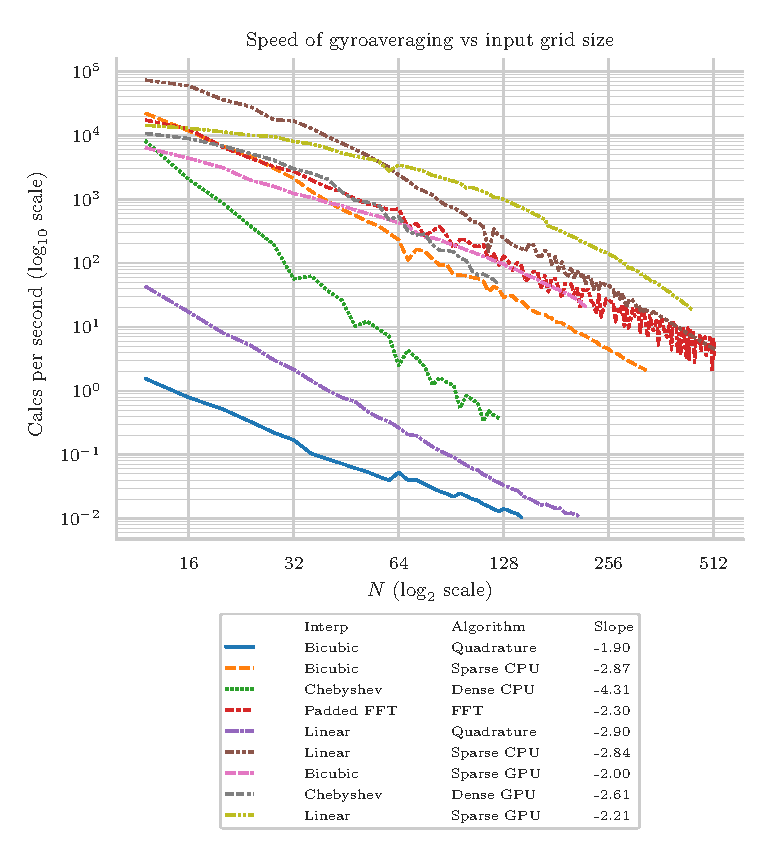
\includegraphics[scale=1]{SpeedVsN.eps}	
 	\caption[Gyroaveraging speed vs grid size]{Calculation speed as grid size grows.  The slope is a linear regression coefficient for the displayed log-log plot.   Note that while the CPU-bound Chebyshev algorithm exhibits worse than quartic scaling, the GPU version scales with lower exponent (-2.61); this reflects the significance of the cost of CPU-GPU memory transfer which scales like $N^2$. }  	\end{figure}
	
	
	\begin{figure}[htbp!]
		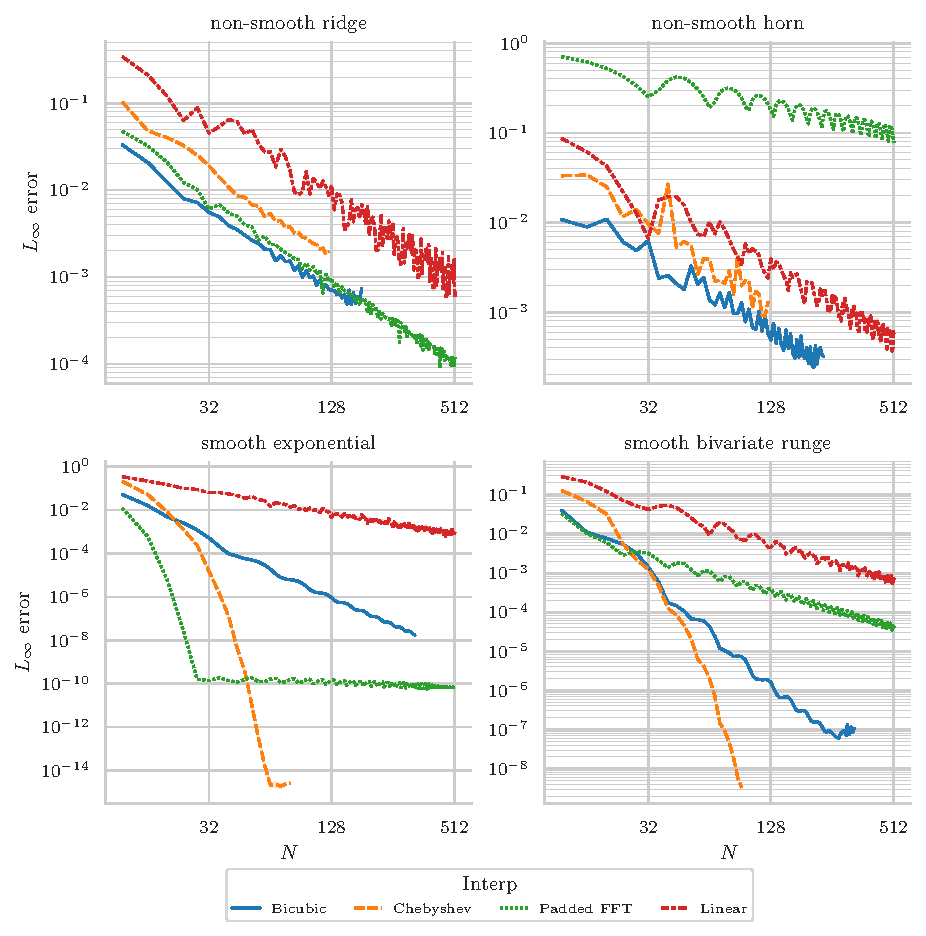
\includegraphics[scale=1]{ConvergenceAllNew.pdf}	
		\caption[Gyroaveraging error vs grid size]{Error vs grid size.  By construction, no one algorithm is a clear winner.  For smooth functions, we get spectral accuracy from the Chebyshev interplation, and the Fourier method as well in the numerically periodic case.}  	\end{figure}

	\begin{figure}[htbp!]
	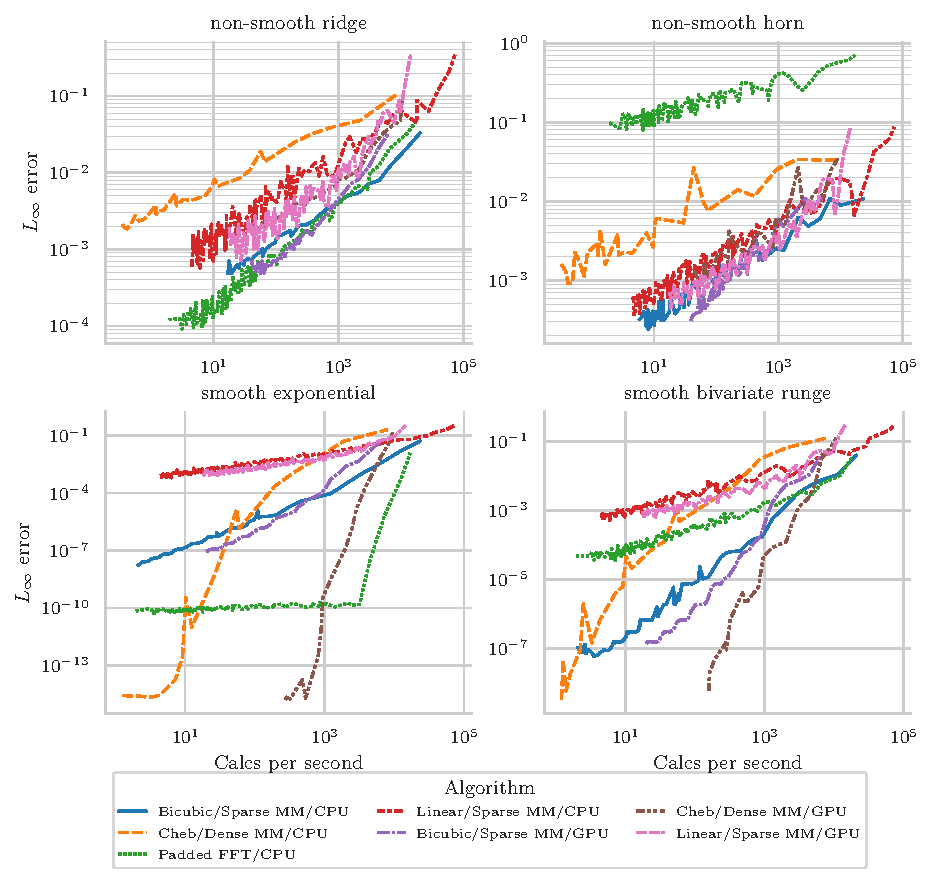
\includegraphics[scale=1]{OptimalAllNew.pdf}	
	\caption{The trade-off between accuracy and execution speed.}  	\end{figure}

	\begin{figure}[htbp!]
	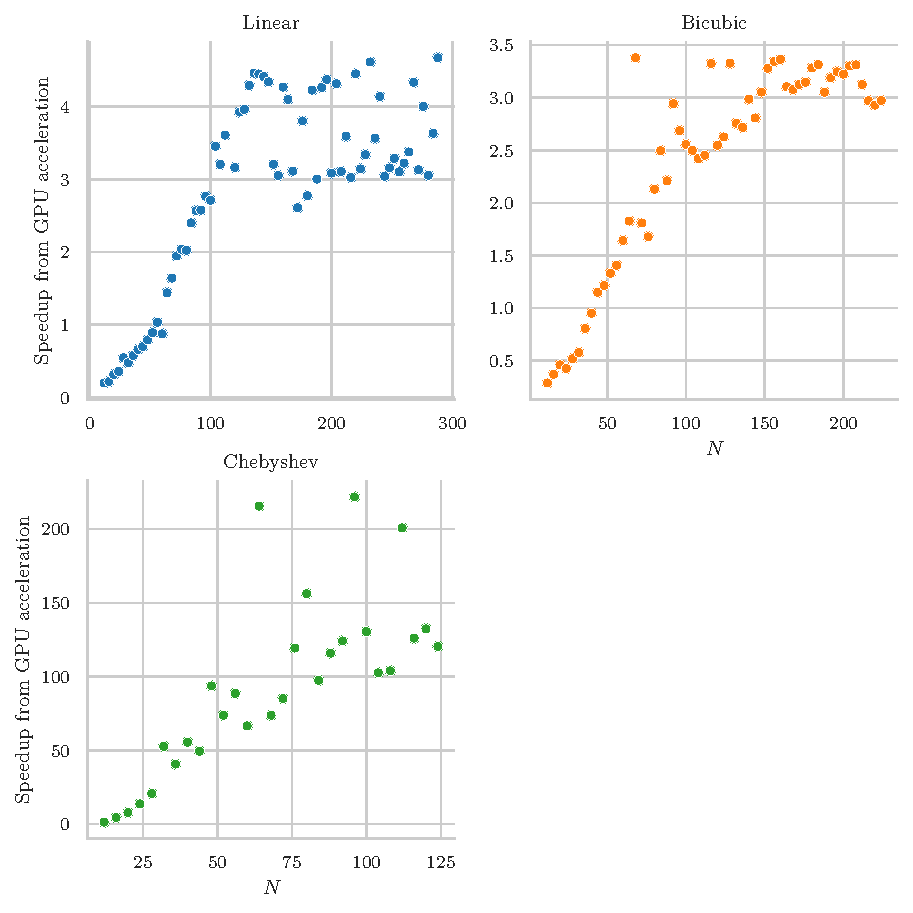
\includegraphics[scale=1]{GPUAccel.pdf}	
	\caption[The benefit from GPU acceleration]{The speed benefit of GPU parallelism.  These acceleration ratios are typical for sparse vs. dense linear algebra.  This includes the full penalty of CPU-GPU memory transfer in both directions.}  	\end{figure}

	
	\section{Discussion of numerical results}  First, as a reference point, it will be useful to refer to \cite[P. 16]{guadagniThesis}.  The author describes a single gyroaverage calculation (for 35 values of $\rho$) of the same ``Smooth Exponential" function we have used, to accuracy $10^{-13}$, taking approximately 13 seconds.  To be clear, \cite{guadagniThesis} was not focused on performance, and notes various potential improvements including parallelization.  
	
	This work has gained 3-4 orders of magnitude performance increase for similar accuracy on this smooth function.  We can trace this to a few different sources, including:  1) Matlab vs C++, 2) multi-core CPU parallelism, 3) GPU acceleration in some cases.
	
	However, both \cite{gorner2012} and \cite{guadagniThesis} present FFT-based methods, which are not expected to converge well for non-smooth functions, nor for functions which are not numerically of compact support.  Except for the ``smooth exponential" function, the bicubic interpolation and Chebyshev based algorithms are competitive with respect to both accuracy and speed with the padded FFT algorithm.  Indeed, as expected, the bicubic interpolation is most robust to the ``horn" singularity.  On the other hand, the Chebyshev interpolation alone is able to demonstrate spectral accuracy for the non-compactly supported ``Runge" function.






\chapter{Conclusion\label{chap:Conclusion}}

\section{Proof of concept}
  We can conclude from the previous chapter three main points:
  \begin{enumerate}
  	\item As a proof of concept, the bicubic and bilinear interpolation schemes for gyroaveraging were successfully translated into sparse linear algebra operations, and parallelized/accelerated using existing state-of-the-art linear algebra libraries.
  	\item These schemes were shown to be competitive with spectral methods when, for instance, singularities make the advantages of spectral methods moot.
  	\item  All methods were implemented efficiently so that $10^3$ gyroaverage calculations could be achieved per second on a single machine (with, admittedly, expensive hardware.)  This required in some cases reframing the discretization so that GPU acceleration could be brought to bear on the problem.
  \end{enumerate}

\section{Further development}
There are many avenues for further testing and development, including:
\begin{enumerate}
	\item Distributed memory parallelism:  Both dense and sparse linear algebra are easily distributed on an HPC grid.  Since the main operation of our algorithms is a single large fixed matrix applied to a relatively small vector, the communication bottleneck should not be severe and all algorithms might scale quite well.
	\item Faster and more accurate precomputation of the dense Chebshev matrix, as described in \ref{chebPrecomp}.
	\item ``Low rank" Chebyshev representations of functions:  The Chebfun2 package, as described in \cite{chebfun2} documents an efficient way to calculate low-rank representations of bivariate functions with the same Chebyshev basis functions we use.  Such low-rank approximations would require only a small portion of the $N^4$ matrix we use, though we would still have to precompute the whole thing.  Easier would be filtering the results of the DCT (i.e. very small Chebyshev coefficients) or, perhaps, throwing out the bottom right half of the Chebyshev coefficients (i.e. high frequency mixed modes.)
	\item Adaptivity.  By using adaptive refinement but on fixed precomputed grids, one could choose the $N$ to approximate the input to some tolerance, and insure a simliar tolerance for the gyroaverages.  This is already non-trivial for the equispaced grids and may not work for Chebyshev.
	\item Integration into a fully GPU workflow: FFTs, finite differencing, and even Poisson solving are all available for GPUs.  For each of the gyroaveraging applications mentioned in the introduction, it is possible that one could avoid GPU-host memory transfer by doing all of the work (including time-stepping or other iteration) on the GPU device.  This is of course very application dependent.
\end{enumerate}


%%%%% Appendices start %%%%%%%%%%%%%%%%
%% Comment out the following line if your thesis has no appendix
%\appendix
%\chapter{One more comment\label{chap:append}}



This is an appendix.

%% Note: If your thesis has more than one appendix, NYU requires a "list of
%% appendices" page before the body of the thesis. I don't provide the tools
%% to create that here, so you're on your own for that one... Sorry.
%\input{app2}
%%%% Input bibliography file %%%%%%%%%%%%%%%
%% Bibliography. I didn't use BibTeX, so you're on your own if you'd like to do so.
%


\printbibliography


%BELOW IS THE OLD BIBLIOGRAPHY STYLE
%\begin{thebibliography}{99}\addcontentsline{toc}{chapter}{Bibliography}
%\bibitem{JBC91}J.~B.~Conway, \emph{Functions of One Complex
%    Variable~I}. Second edition. Springer-Verlag, Graduate
%    Texts in Mathematics~\textbf{11}, 1991.
%\end{thebibliography}


\end{document}
